\documentclass[10pt, a4paper]{article}

\usepackage{comment} % enables the use of multi-line comments (\ifx \fi)
\usepackage{amsmath}
\usepackage[left=0.7cm,right=0.7cm,top=0.5cm,bottom=0.7cm,includehead,
headheight=0.7cm, headsep=0.3cm]{geometry}
\usepackage[indent=0cm]{parskip}
\usepackage{enumitem}
\usepackage{graphicx}
\usepackage{titlesec}
\usepackage{booktabs}
\usepackage{fancyhdr}
\usepackage{lastpage}
\usepackage[english]{babel,varioref}
\usepackage{enumitem}
\setlist{nosep}
\setlist{leftmargin=*}

% Document information
\newcommand{\titleinfo}{TSM\_AnSeqDa -- Analysis of Sequential Data}
\newcommand{\authorinfo}{Selvin Blöchlinger}
\newcommand{\version}{1.0}
\newcommand{\versioninfo}{HS24}

% Spacing
\titlespacing{\section}{\parskip}{1pt}{1pt}
\titlespacing{\subsection}{\parskip}{1pt}{1pt}
\titlespacing{\subsubsection}{\parskip}{1pt}{1pt}

% Header / Footer
\pagestyle{fancy}
\fancyhf{}
\fancyhead[L]{\titleinfo{ }\tiny{(\versioninfo{ V}\version)}\normalsize\qquad\authorinfo{ }}
\fancyhead[R]{Page{ }\thepage{ }of{ }\pageref{LastPage}}

% Math Operators
\DeclareMathOperator{\var}{var}
\DeclareMathOperator{\mean}{mean}
\DeclareMathOperator{\E}{E}
\DeclareMathOperator{\I}{\mathcal{I}}
\DeclareMathOperator{\floor}{floor}
\DeclareMathOperator{\MSE}{MSE}
\DeclareMathOperator{\MAE}{MAE}
\DeclareMathOperator{\MAPE}{MAPE}
\DeclareMathOperator{\RMSE}{RMSE}
\DeclareMathOperator{\MASE}{MASE}
\DeclareMathOperator{\SSE}{SSE}
\DeclareMathOperator{\AR}{AR}
\DeclareMathOperator{\MA}{MA}


\begin{document}


\section{Stochastic Processes}
A stochastic process (SP) is a sequence of random variables indexed in time order: $ Y_1, Y_2, Y_3, ..., Y_t $.
Realization of a stochastic process yield a time series.
Taking a sample from the stochastic process means sampling a possible future behaviour of the system.
Using only past data to predict a future is hard, which is why a model of the system behaviour is chosen first.
We then try to predict a new value given past observations as $ Y_t | Y_{t-1} = Y_t | Y_1, Y_2, ... Y_{t-1} $. Time series can exhibit three major patterns:

Trend: pattern exists when there is a long-term increase or decrease in the data.

Seasonal: pattern exists when a series is influenced by seasonal factors in a predictable and fixed way.

Cyclic: pattern exists when data exhibit rises and falls that are not of fixed period

\section{Autocorrelation}
(Linear) Correlation of random variables of a time series at different times: $ AutoCorr(t_1, t_2) = Cor(X_t{_1}, X_{t_2}) $.
Plotting the autocorrelation for different time lags produces a correlogram or Autocorrelation Function (ACF).
Seasonality can be seen by high positive values at lags that are multiples of the seasonality; a trend can be seen by higher absolute values for small lags.
A time series with both patterns will show a mix of both in the ACF. White noise series will produce values below the critical threshold of $ \pm 1.96 / \sqrt{T} $ for all lags.

\section{Statistical Hypothesis Testing (SHT)}
SHT is toolbox to decide if given data supports a particular given hypothesis.
It works by choosing a null hypothesis, e.g. the time series is white noise.
We then choose a statistical test, e.g. Ljung‐Box and compute its test statistics for a given signifance level, e.g. 5\%.
If the p-Value is very small, that means it is very unlikely to sample a series this extreme given the null hypothesis. We thus reject the hypothesis.

\section{Forecasting}
Computation of forecast at different points in time with $ \hat{y}_{t|t-1} $ as the fitted value of $ y $ at time $ t $ given past values up to time $ t - 1 $.
We can perform $ h-$ step forecasts by iteratively applying one step forecasts.
Often, a model is chosen that is well suited to the characteristics of the time series and then fitted to it. This model can then be used to perform forecasts.

\subsection{Simple Forecast Methods}
Average: Forecast of all future values is equal to mean of historical data.

Naïve: Forecast of all future values is equal to the last observed value.

Seasonal Naïve : Forecast of all future values is equal to the last observed value from the same season.

Drift: Forecast equal to last value plus average change in historical values. Results in a straight line between last observed and last forecasted values.

\subsection{Residual Analysis}
Residuals in forecasting are defined as the difference between observed value and its fitted value: $ e_t = y_t - \hat{y}_{t|t-1} $.
Residuals should have zero mean. If they do not, the forecast performed with the fitted model is biased. The should also be uncorrelated.
If they are not, the residuals contain information not captured by the fitted model. Residuals are also assumed to have constant variance and to be normally distributed.

\subsection{Evaluating Forecast Accuracy}
The residuals produced by fitting a model should be indistinguishable from white noise by fulfilling all criteria above.
We can use SHT with a test like Ljung Box to test whether this is true.
Small p-values lead to rejecting the null hypothesis meaning residuals are correlated.
Having small residuals does not guarantee good forecasting performance.

Forecast Errors are also used for evaluating forecasts. The data is split into a training and a test set.
The training set is used for fitting the chosen model while the test set is used to evaluate its performance.
Based on the test set containing $ n $ values, different error metrics can be computed:
$ MAE = \frac{1}{n} \sum_{i=1}^{n} |y_i - \hat{y}_i| $,
$ MSE = \frac{1}{n} \sum_{i=1}^{n} (y_i - \hat{y}_i)^2 $,
$ MAPE = \frac{1}{n} \sum_{i=1}^{n} \left| \frac{y_i - \hat{y}_i}{y_i} \right| \times 100 $,
$ RMSE = \sqrt{\frac{1}{n} \sum_{i=1}^{n} (y_i - \hat{y}_i)^2} $,
$ MASE = \frac{1}{n} \sum_{i=1}^{n} \frac{|y_i - \hat{y}_i|}{\frac{1}{n-1} \sum_{i=2}^{n} |y_i - y_{i-1}|} $,
$ SSE = \sum_{t=1}^{n} (y_t - \hat{y}_t)^2 $.
$ MAE $, $ MSE $, $ RMSE $ and $ SSE $ are all scale dependent.
$ MAPE $ is scale independent but is only sensible if $ y_t \gg 0 \text{ for all } t $, and $ y $ has a natural zero.

Cross-validation for time series involves iteratively splitting a time-ordered dataset into training and test sets,
ensuring that the test set comes after the corresponding training set,
to assess the performance of a model on multiple folds and mitigate the risk of temporal information leakage
(giving the model access to the future it is supposed to predict).

\subsection{Prediction Intervals}
A prediction interval gives a region within which we expect the forecast value with a specific probability.
It serves as a measure of confidence in the prediction. The 95\% prediction interval for an $ h $-step forecast can be computed
as $ \hat{y}_{T+h|T} \pm 1.96 \hat{\sigma}_h $, with $ \hat{\sigma}_h $ as the stddev of the $ h $-step distribution.
Assuming the residuals are normally distributed, $ \hat{\sigma}_h $ can be estimated for different forecast methods as:

$ \text{Mean: } \hat{\sigma} \cdot \sqrt{1+1/T}, \text{Naïve: } \hat{\sigma} \cdot \sqrt{h},
\text{Seasonal Naïve: } \hat{\sigma} \cdot \sqrt{k+1}, \text{Drift: } \hat{\sigma} \cdot \sqrt{h \cdot (1+h/T)} $
where $ \hat{\sigma} $ is the stddev of the residuals, $ T $ is the number of historical values, $ h $ is the integer part of $ (h-1)/m $ and $ m $ is the seasonal period.

\section{Exponential Smoothing}
Exponential smoothing is a time series forecasting method that assigns exponentially decreasing weights to past observations,
providing a weighted average of historical data to generate a smoothed forecast with a focus on recent trends.
Parameters such as $ \alpha $ or $ \phi $ can be found via optimization of the $ SSE $.

\subsection{Simple Exponential Smoothing (SES)}
A a weighted moving average, whose weights decrease exponentially:
$ \hat{y}_{t} = \alpha \cdot y_{t-1} + \alpha \cdot (1 - \alpha) \cdot \hat{y}_{t-1} + \alpha \cdot (1 - \alpha)^2 \cdot \hat{y}_{t-2} + ... $
where $ 0 \le \alpha \le 1 $. The weights sum up to one as a geometric series.
SES provides flat forecasts for all time horizons as it does not incorporate any trend or cyclic components.

Forecast Equation: $ \hat{y}_{t+h|t} = \ell_t $;
Smoothing Equation: $ \ell_t = \alpha \cdot y_t + (1 - \alpha) \cdot \ell_{t-1} $

\subsection{Trend Methods}
\textbf{Holt's linear trend}
Forecast Equation: $ \hat{y}_{t+h|t} = \ell_t + h \cdot b_{t-1} $;
Smoothing Equation: $ \ell_t = \alpha \cdot y_t + (1 - \alpha) \cdot (\ell_{t-1} + b_{t-1}) $;
Trend Equation: $ b_t = \beta \cdot (\ell_t - \ell_{t-1}) + (1 - \beta) \cdot b_{t-1} $

\textbf{Holt's linear with damped trend}
Forecast Equation: $ \hat{y}_{t+h|t} = \ell_t + h \cdot \phi \cdot b_{t-1} $;
Smoothing Equation: $ \ell_t = \alpha \cdot y_t + (1 - \alpha) \cdot (\ell_{t-1} + \phi \cdot b_{t-1}) $;
Trend Equation: $ b_t = \beta \cdot (\ell_t - \ell_{t-1}) + (1 - \beta) \cdot \phi \cdot b_{t-1} $

\subsection{Seasonal Methods}
Holt-Winters is an extension to Holt's method to capture seasonality.

\textbf{Additive:} seasonality component is constant

Forecast Equation: $ \hat{y}_{t+h|t} = \ell_t + hb_{t-1} + s_{t-m+h-m(q+1)} $;
Smoothing Equation: $ \ell_t = \alpha (y_t - s_{t-m}) + (1 - \alpha)(\ell_{t-1} + b_{t-1}) $;
Trend Equation: $ b_t = \beta (\ell_t - \ell_{t-1}) + (1 - \beta) b_{t-1} $;
Seasonality Equation: $ s_t = \gamma (y_t - \ell_{t-1} - b_{t-1}) + (1 - \gamma) s_{t-m} $;

\textbf{Multiplicative}: seasonality component is proportional to series level

Forecast Equation: $ \hat{y}_{t+h|t} = (\ell_t + hb_{t-1}) \cdot s_{t-m+h-m(q+1)} $;
Smoothing Equation: $ \ell_t = \alpha \frac{y_t}{s_{t-m}} + (1 - \alpha)(\ell_{t-1} + b_{t-1}) $;
Trend Equation: $ b_t = \beta (\ell_t - \ell_{t-1}) + (1 - \beta) b_{t-1} $;
Seasonality Equation: $ s_t = \gamma \frac{y_t}{\ell_{t-1} + b_{t-1}} + (1 - \gamma) s_{t-m} $;

\subsection{Exponential Smoothing State Space Models (ETS)}
Contrary to pure forecasting methods, State Space Models can provide point forecasts as well as prediction intervals.
They assume three components that make up the time series:

Error: {Additive, Multiplicative}

Trend: {None, Additive, Additive damped}

Sesonal: {None, Additive, Multiplicative}

\noindent
Automatic Forecasting aims to find the best performing model out of all possible permutations above by choosing
the model with the lowest $ AIC = -2 \ln(\mathcal{L}) + 2k $ or $ AICc = AIC + \frac{2k(k+1)}{n-k-1} $,
where $ \mathcal{L} $ is the likelihood of the model, $ k $ is the number of estimated parameters in the model and $ n $ is the number of observations.

\section{Autoregressive Integrated Moving Average (ARIMA)}
Combines autoregressive (AR) and moving average (MA) components along with differencing (I).

\subsection{Random Walk (with drift)}
$ y_t = c + y_{t-1} + \epsilon_t $

\subsection{Stationarity}
Refers to a time series property where statistical properties, such as mean and variance, remain constant over time,
providing a stable and predictable behavior. Stationary processes drop quickly to zero and no seasonality visible in the ACF.
Non-stationary processes decrease more slowly or not at all.

\subsection{Differencing}
Change between observations in the time series. Can be done multiple times or for observations in the same season.
Differencing can help with obtaining a stationary time series. Finding the correct number of differences to obtain stationarity can be automated.
Backshift notation: $ By_t = y_{t-1} \text{; } y_t' = y_t - y_{t-1} = (1 - B) \cdot y_t \text{; } y_t'' = (1 - B)^2 \cdot y_t$

\subsection{Autoregressive (AR) and Moving Average (MA) models}
Autoregressive Models use multiple regression with lagged values of $ y_t $ as predictors:
$ y_t = c + \phi_1 y_{t-1} + \phi_2 y_{t-2} + \ldots + \phi_p y_{t-p} + \varepsilon_t $, denoted as AR(p)

They work only on stationary data. All $ \phi $ values are restricted such that the complex roots of the characteristic polynom lie outside the unit circle.

Moving Average Models use multiple regression with past noise as predictors:
$ y_t = c + \varepsilon_t - \theta_1 \varepsilon_{t-1} - \theta_2 \varepsilon_{t-2} - \ldots - \theta_q \varepsilon_{t-q} $, denoted as MA(p)

Any $ MA(q) $ process can be written as an $ AR(\infty) $ when the roots of the characteristic polynom lie outside the unit circle.

\subsection{ARMA and ARIMA models}
ARMA: $ y_t = c + \phi_1 y_{t-1} + \phi_2 y_{t-2} + \ldots + \phi_p y_{t-p} + \theta_1 \varepsilon_{t-1} + \theta_2 \varepsilon_{t-2} + \ldots - \theta_q \varepsilon_{t-q} $

ARIMA: Combine ARMA with differencing; p = order of the autoregressive part; d = degree of first differencing involved; q = order of the moving average part


\section{Digital Signals}
Complex exponential sequence: \(x(n) = Ae^{j(\omega_0n+\varphi)} = A \cos(\omega_0n+\varphi) + jA\sin(\omega_0n+\varphi)\),
with \(\omega_0=\frac{2\pi}{T_0}=2\pi f_0 = 2 \pi \frac{f}{f_s}\)

\textbf{Discrete Fourier Series}: \(\displaystyle \ x(n)=\frac{1}{N}\sum_{k=0}^{N-1}X(k)e^{j\overbrace{(2\pi/N)k}^{\omega_0(k)}n}
\ \Leftrightarrow \ X(k)=\sum_{k=0}^{N-1}x(n)e^{-j(2\pi/N)kn} = \textstyle X(f{=}\frac{f_s k}{N})
\quad( 0 \le k,n < N)\)

\begin{minipage}[t]{0.49\textwidth}
    \textbf{DFT properties}\\
    \begin{tabular}{@{}lll@{}}\toprule
        Property & Time Domain & Frequency Domain \\ \midrule
        Periodicity & \(x(n) = x(n+N)\) & \(X(k) = X((k))_N\) \\
        Linearity & \(ax_1(n) + bx_2(n)\) & \(aX_1(k) + bX_2(k)\) \\
        Convolution & \(x_1(n) * x_2(n)\) & \(X_1(k) X_2(k)\) \\
        Multiplication & \(x_1(n) x_2(n)\) & \(\frac{1}{N}(X_1(k) * X_2(k))\) \\
        \bottomrule
    \end{tabular}
\end{minipage}
\hfill
\begin{minipage}[t]{0.49\textwidth}
    \textbf{LTI systems}\\
    Output: \(y(n) = \sum_{k=-\infty}^{\infty}x(n)h(n-k) = x(n) * h(n)\)\\
    Frequency response \(H(\omega)\): \(Y(\omega)=X(\omega)H(\omega)\)\\
    FIR Filter: \(y(n)=a_0x(n) + a_1x(n-1) + \cdots + a_px(n-p)\)
\end{minipage}


\section{Speech Signals}
\textbf{Information content}: What?, Who?, How?, speaking environment, transmission channel, background noise

\textbf{Phonemes}: Smallest sound unit, speaker-independent. Western languages have 20 to 60 phonemes (German: 48).\\
\textbf{Phones}: Acoustic representation of the phoneme, speaker-dependent.

\textbf{Short-time spectral analysis}: Calculate the spectrum of a sliding window.
Idea: speech signal is quasi-stationary inside the window.
Spectrum of the windowed signal: \(\bar{X}(\omega)=X(\omega)*W(\omega)\).
Smoother window \(\leftrightarrow\) lower side lobes. Longer window \(\leftrightarrow\) higher spectral resolution.
The \textbf{Spectrogram} shows the temporal changes in the signal spectrum.

\textbf{Formants} are high energy areas in the spectrogram (usually dark).
The fundamental frequency \(F_0\) ranges from 50~Hz (deep mans voice) to 400~Hz (child), depending on the speaker.
The formants \(F_1\) to \(F_4\) convey information about the phone sequence.
\(F_1\) and \(F_2\) are speaker dependent.

\begin{minipage}[t]{0.35\textwidth}
\centering
\textbf{Vowels}
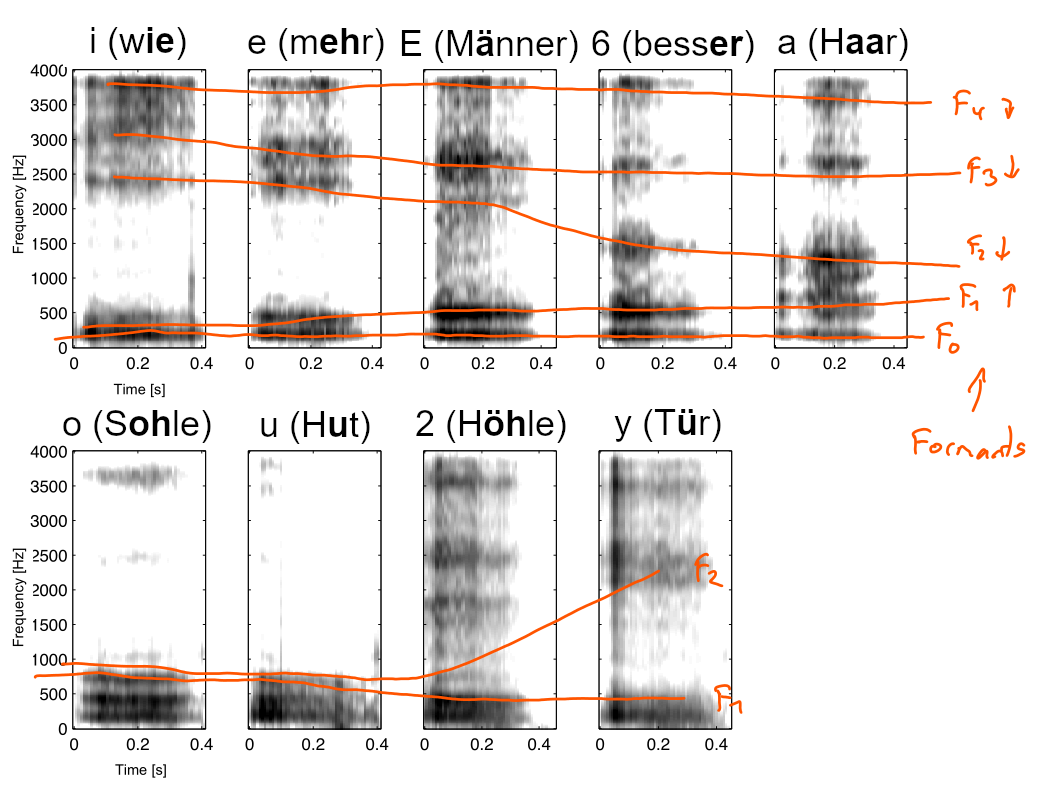
\includegraphics[width=\textwidth]{img/vowels}
\textbf{Diphthongs}
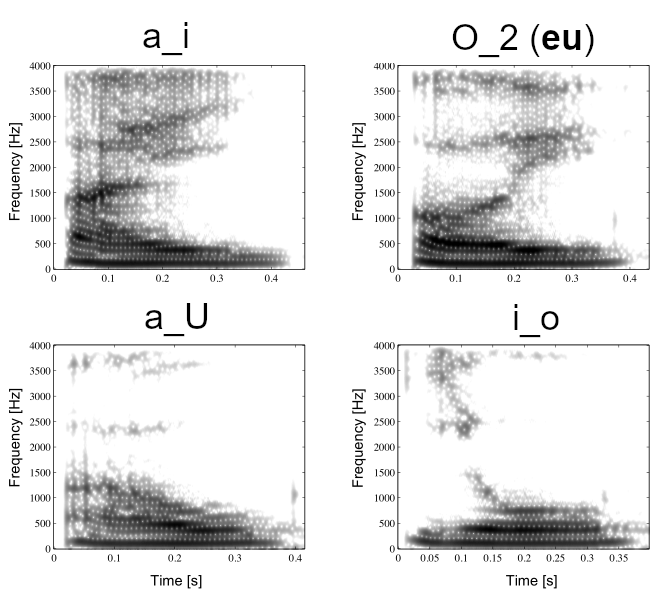
\includegraphics[width=0.9\textwidth]{img/diphthongs}
\end{minipage}
\hfill
\begin{minipage}[t]{0.31\textwidth}
\centering
\textbf{Fricatives (unvoiced)}
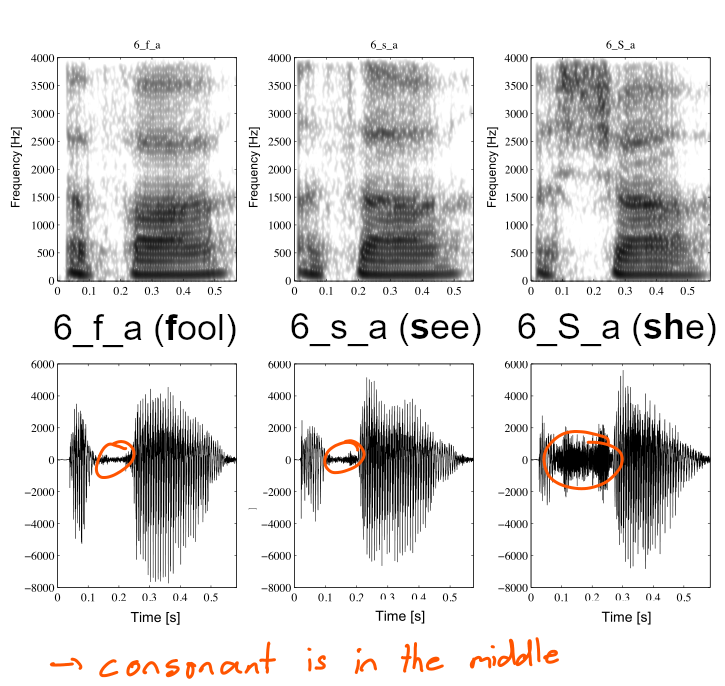
\includegraphics[width=\textwidth, trim={0 0 0 3mm}, clip]{img/fricatives_unvoiced}
\textbf{Nasals / Laterals}
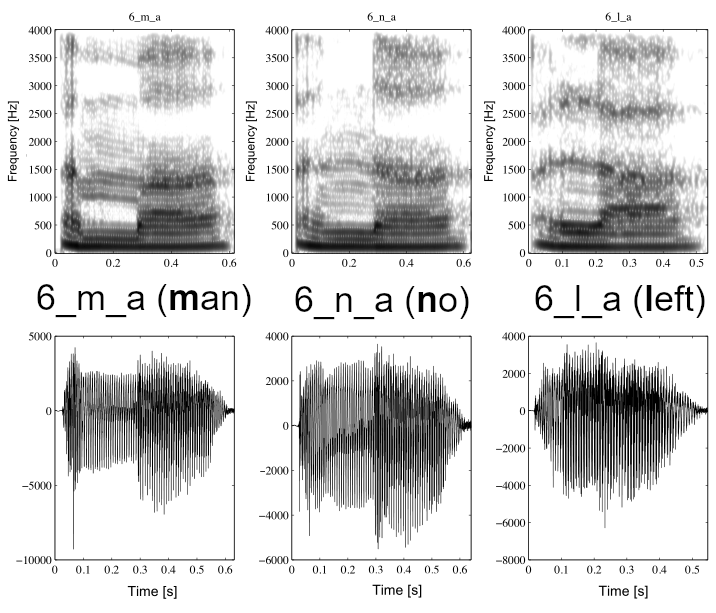
\includegraphics[width=\textwidth]{img/nasals_laterals}
\end{minipage}
\hfill
\begin{minipage}[t]{0.32\textwidth}
\centering
\textbf{Plosives (voiced)}
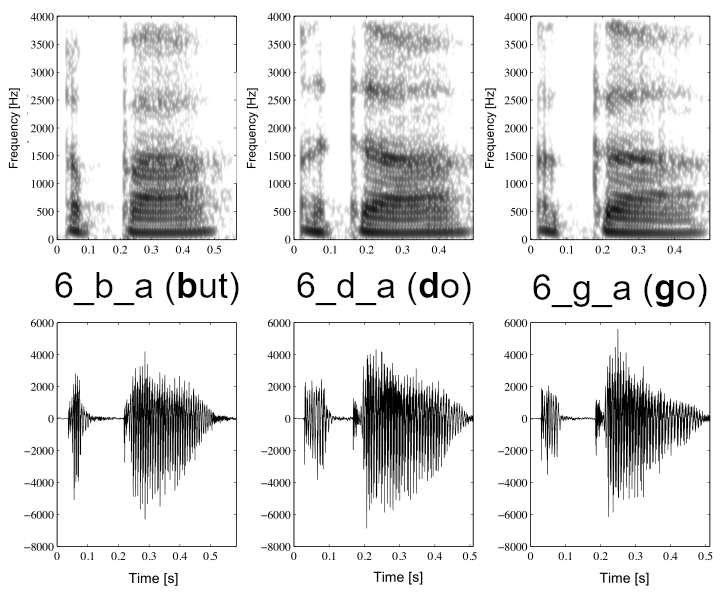
\includegraphics[width=\textwidth]{img/plosives_voiced}
\textbf{Plosives (unvoiced)}
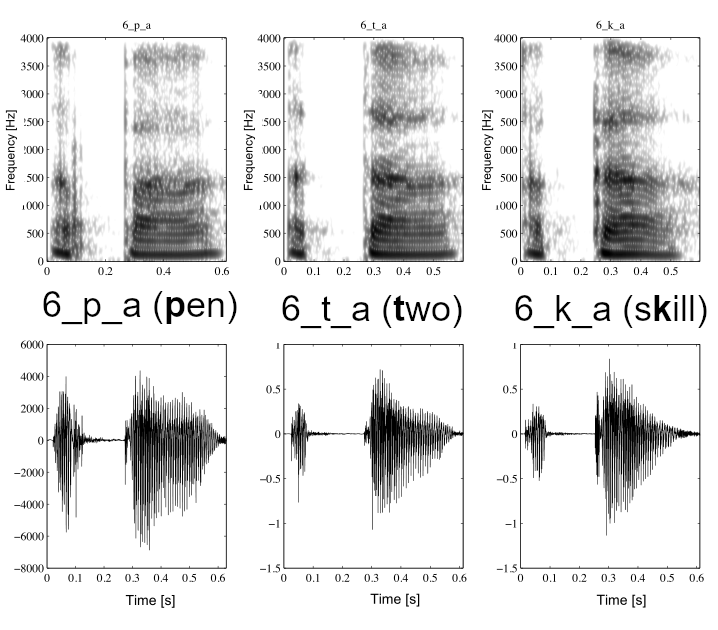
\includegraphics[width=\textwidth]{img/plosives_unvoiced.png}
\end{minipage}


\begin{minipage}[]{0.49\textwidth}
\centering
\textbf{Utterance of ``Sieben''} with \(F_0=100\)~Hz (male)
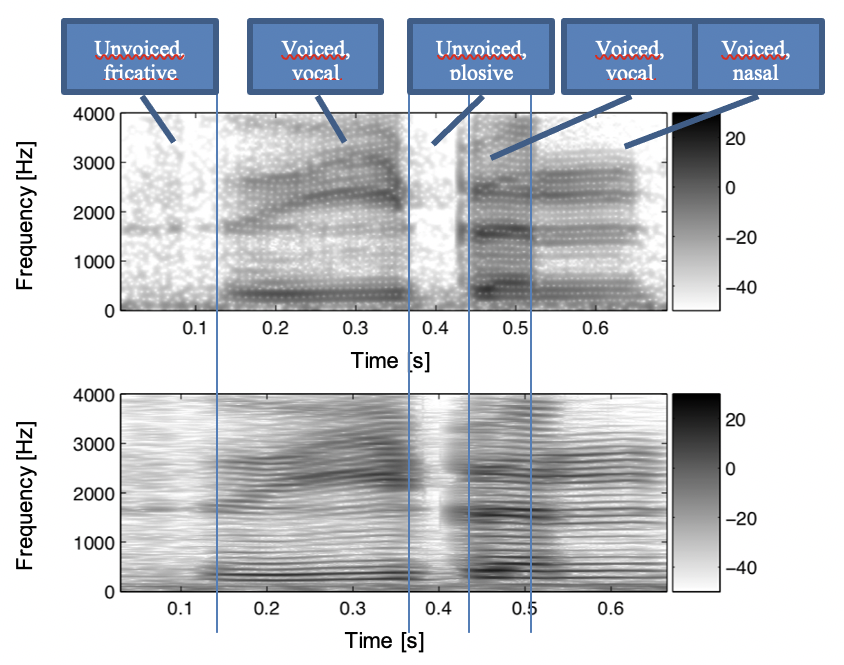
\includegraphics[width=\linewidth]{img/spectrogram_sieben}
\end{minipage}
\hfill
\begin{minipage}[]{0.4\textwidth}
\centering
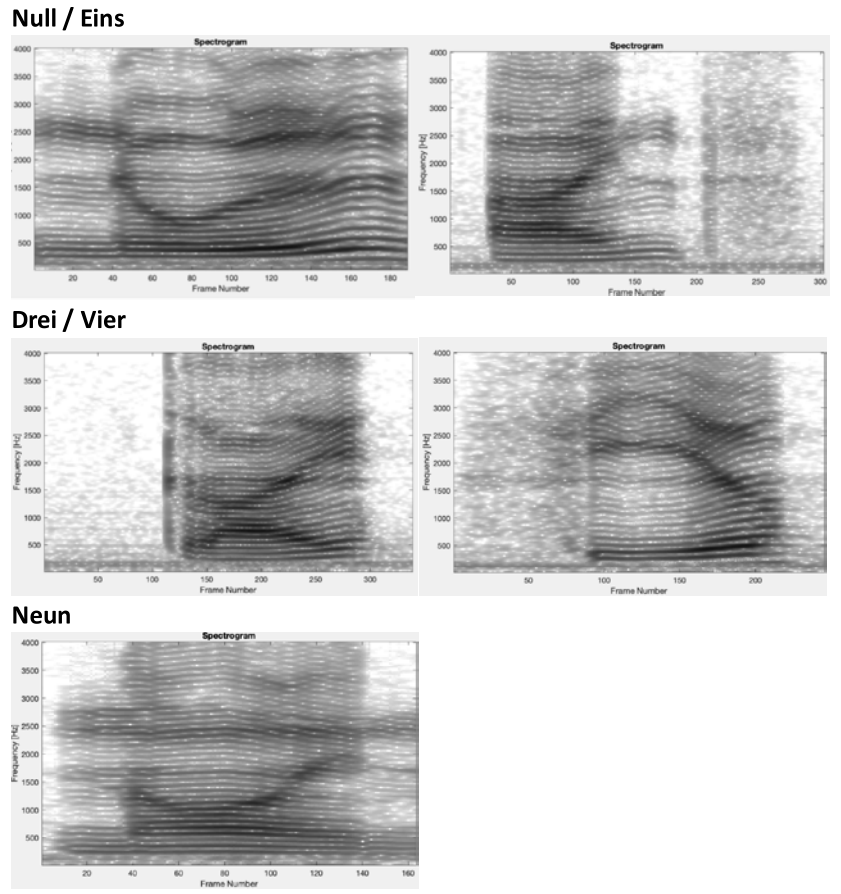
\includegraphics[width=\linewidth]{img/german_digits}
\end{minipage}


\subsection{Speech Recognition}
Speech recognition is the technology that converts spoken language into written text,
allowing computers to understand and process verbal commands or transcribe spoken words.
Very difficult because human voices can be very different, humans make mistakes, background noises and different acoustics for different environments.
Also, there are no word boundaries in human speech.

\subsubsection{Feature Extraction}
For speech recognition, spectrograms and the formants are important features.
Unimportant information can be filtered out by many means,
e.g. DFT-Cepstrum (IDFT of the Log of the DFT-Spectrum) to extract the source (vocal excitation) from the filter (vocal tract) components.
A Mel-Spectrum is a spectrum that more closely resembles the characteristics of the human ear by having logarithmic sensitivity
for frequencies above 1~kHz (lower sensitivity for higher frequencies).
Mel-Cepstrum: IDFT of Log(Mel-Spectrum). The Fast Cochlea Transform (FCT) is a signal processing technique inspired by the auditory processing in the human cochlea.

\subsubsection{Classical Approaches: Rule- based and Pattern Matching}
Both require feature extraction from the speech signal.

Rule- based: Classification is based on rules for each class derived from human knowledge/observation.
Very difficult because not generalizable for different speakers.

Pattern Matching: Classification based on a distortion measure between a feature pattern and given reference patterns for each class (kNN, SVMs).
Main problem is that the patterns can also vary in the temporal structure.
We can use Dynamic Time Warping (DTW) to align the extracted features to the reference features by
locally stretching or squeezing pattern by duplicating or dropping feature vectors.

\subsubsection{Statistical Classification}
To calculate joined probabilities, we can use bayes rule: $ P(X | W) = \frac{P(W | X) \cdot P(W)}{P(X)} $

Given extracted feature  $ X $ from the speech recognizer, the MAP classifier must choose the word sequence $ W $
that has the highest a-posteriori probability of all possible word sequences.

\subsubsection{Hidden Markov Model (HMM)}
Defined by N states, state transition probabilities as well observation probability distribution in each emitting state.

Forward Algorithm: Given a HMM $ \lambda $, a sequence of emitted observations $ \textbf{X} = x_1, x_2, \ldots, x_T $,
we want to efficiently calculate $ P(\textbf{X} | \lambda) $. Known as Evaluation problem.
Brute force approach would be to simply try out all state combinations and see which one has the highest likelihood of giving the seen sequence.
Forward algorithm takes advantage of independent states and instead keeps the probabilities for emitting the observations for each state. Forward: Addition.

Viterbi Algorithm: Given a HMM $ \lambda $, a sequence of emitted observations $ \textbf{X} = x_1, x_2, \ldots, x_T $,
we want to efficiently calculate the most likely state sequence $ Q* = \max_Q P(Q | \textbf{X}, \lambda) $.
Known as Decoding Problem. Same idea as Forward, but instead of adding all possibilities, we always take the max.
N-best Viterbi outputs the N-best state sequences instead of only the best.

Forward-Backward algorithm/Baum-Welch algorithm: Given a sequence of emitted observations $ \textbf{X} = x_1, x_2, \ldots, x_T $ and a model structure,
find parameters for HMM $ \omega $ such that $ \omega* = \max_{\lambda} P(\textbf{X} | \lambda) $.
Known as Estimation Problem. How HMMs are trained.
Forward-Backward estimates the probabilities of the sequence given the current models while Baum-Welch applies changes to optimize the parameters,
kind of like backpropagation.

\subsubsection{HMM Speech Recognizer}
Speech recognition is done with HMMs of sub-units that are concatenated to word and sentence recognition networks.
Viterbi then finds the most likely path through the network.
State sequence $ \xrightarrow{} $ subunit sequence $ \xrightarrow{} $ word sequence $ \xrightarrow{} $ sentence

Lexicon: Describes pronounciation of all words allowed; Language model: Describes all utterances allowed and their probabilities.
Typically, Mel-Cepstrum, Delta-Cepstrum or other are used as features.

Disadvantages: HMM assumptions never totally met in practice: Conditional independence of states and observations;
Training HMMs is not inherently discriminative but rather likelihood maximizing.

\subsubsection{Deep Learning Speech Recognizer}
\textbf{Datasets}: Split dataset into training and test/evaluation sets.
\textbf{Word Error Rate}: Count substitutions (S), insertions (I), deletions (D) and divide by number of words in ground truth.
\textbf{Data Preprocessing} Scale input data to have zero mean and unit variance.
\textbf{Initialization}: use random gaussian distributed weights.
\textbf{Overfitting}: Memorizing the training set. Use dropout to mitigate.
\textbf{Batch Size}: Compromise between faster and more optimal training.
\textbf{Batch Normalization}: Scale the activations to have zero mean and unit variance (only during training).

Normal Depp Neural Networks (DNN) classify only input patterns of constant size (e.g. image), so other architectures are used.

\textbf{DNN-HMM}: Use DNN as feature extractor for HMM; \textbf{CNN}: Use CNN on spectrogram;
\textbf{LSTM vs. GRU}: both types of recurrent neural network (RNN) architectures designed to address the vanishing gradient problem in traditional RNNs.
LSTMs have a more complex memory cell that consists of a cell state and three gates - input gate, forget gate, and output gate.
GRUs have a simpler memory cell with two gates - reset gate and update gate.


\end{document}
